\section{Programs Structure}\label{S_Program}
The files, the directory must contain, are listed in chapter~\ref{SS_1stSteps}. The Python script \emph{Pyrolysis.py} accesses to all the defined classes and controls the whole PKP program. So PKP can be launched the simplest way by starting \emph{Pyrolysis.py}.\\
The figure~\ref{F_Structure} gives a overview of the program structure.\\

The whole program structure is visualized in figure~\ref{F_Structure}, the fitting structure in figure~\ref{F_OptimizationProc}. For a detailed documentation for each class and its method, see the document \emph{PKP Code Documentation}.\\
All required Python packages are also listened in this document.\footnote{For Windows it is easier to install Python(x,y) (https://code.google.com/p/pythonxy/) which includes all these packages than install each of them manually.}

\begin{figure}
\centering%\capstart
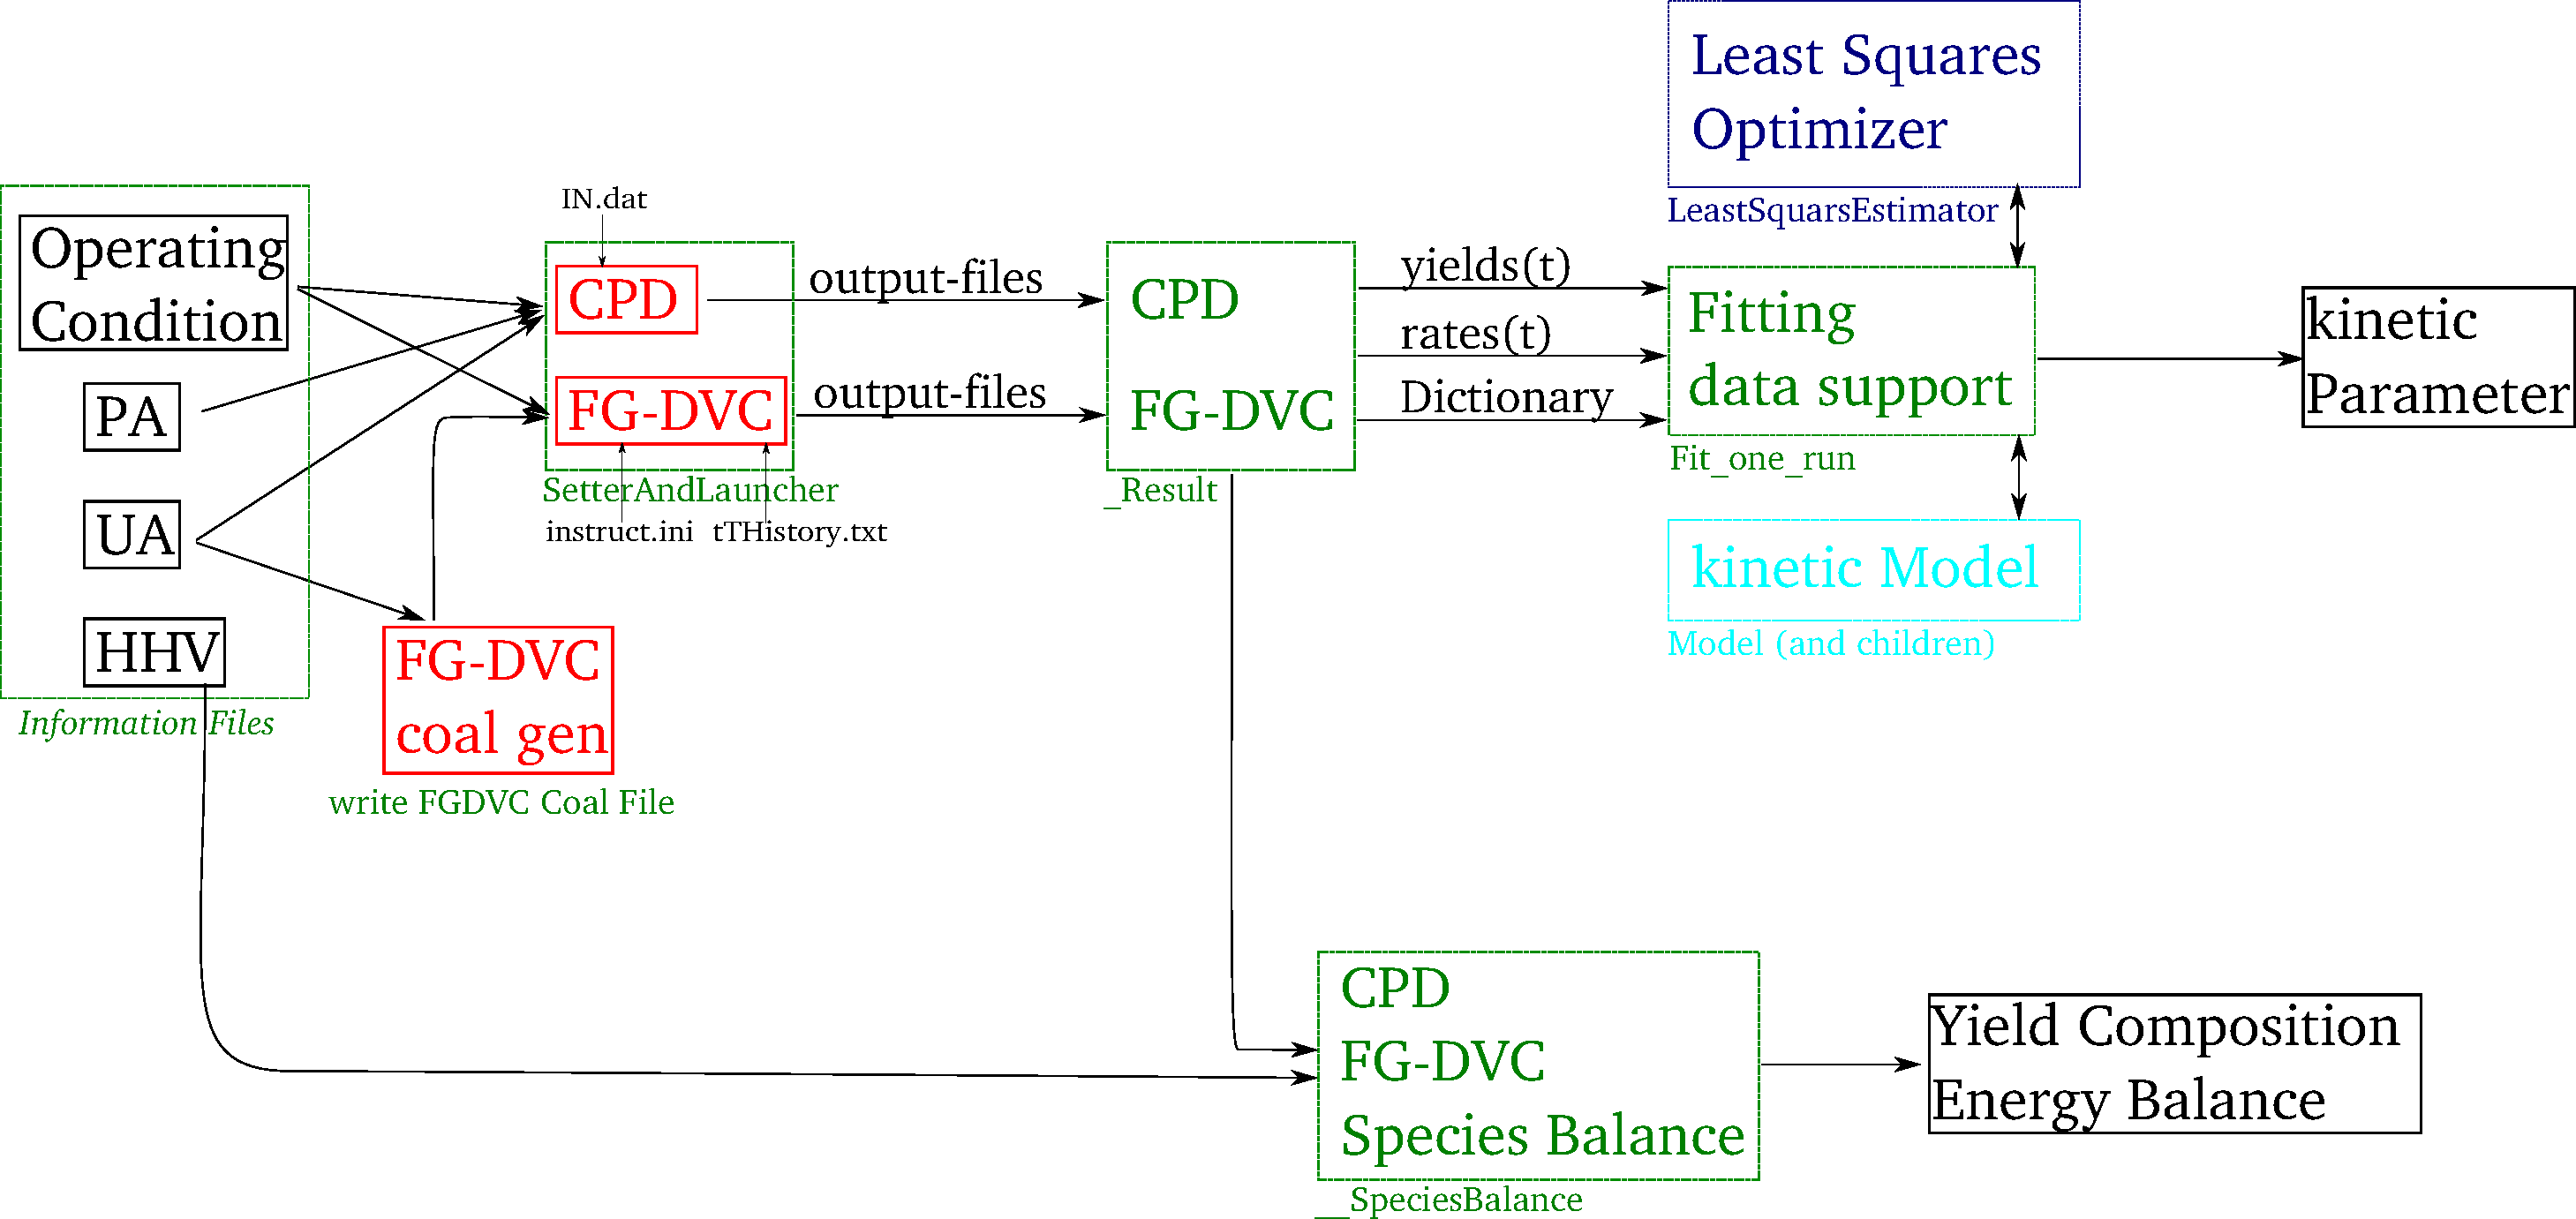
\includegraphics[width=22cm,angle=90]{Figures/Programstructure}
\caption{Overview of the program. The Optimization procedure is shown detailed in figure~\ref{F_OptimizationProc}.}
\label{F_Structure}
\end{figure}

\begin{figure}
\centering%\capstart
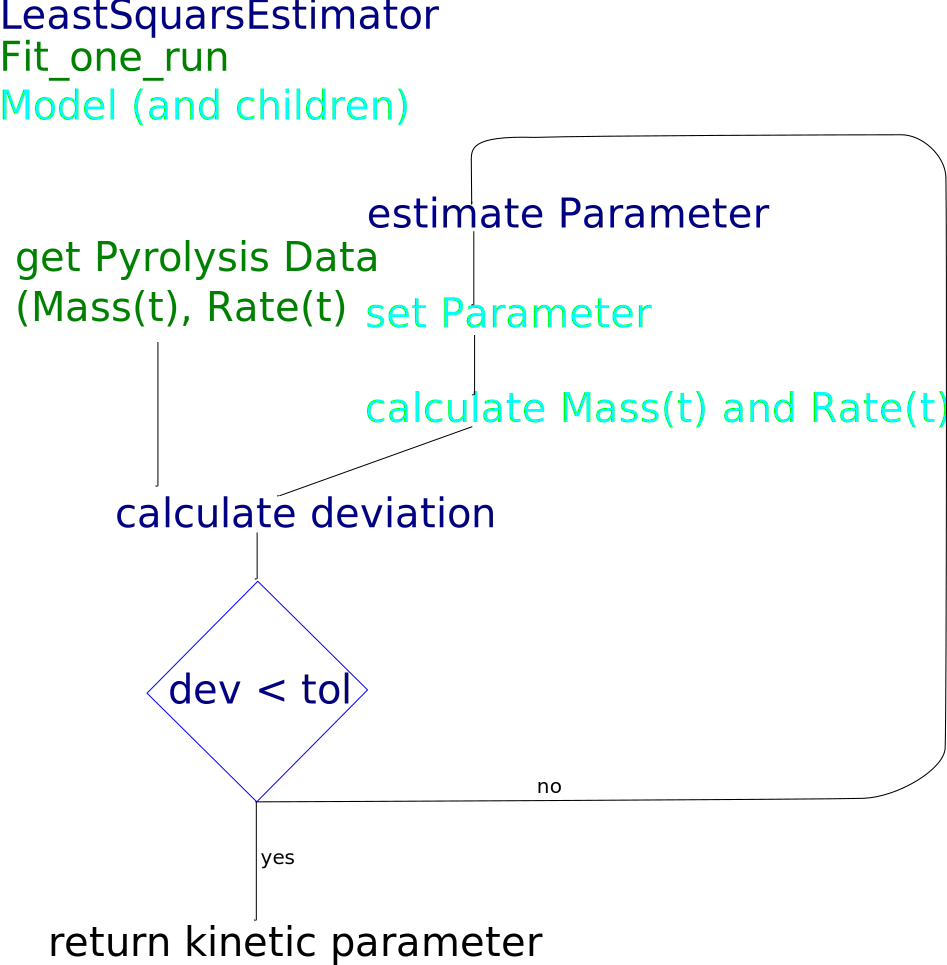
\includegraphics[height=9cm,angle=0]{Figures/FittingProcedure}
\caption{The optimization structure. The three classes \textit{LeastSquarsEstimator}, \textit{Fit\_one\_run} and \textit{Model} are marked with different colors like in Figure~\ref{F_Structure}. The Deviation is calculated with equation~\ref{E_LS}.}
\label{F_OptimizationProc}
\end{figure}

In figure~\ref{F_Structure} the external programs are colored in red, the PKP classes are in green, marked below with the class name or the relevant file name. Inputted, transfered or outputted data is in black.\\
So as first the specific user information about the operating conditions and the coal properties are imported using the reading classes contained in \emph{Information Files.py}.\\
Parts of this information are further used to write the input file for the \FGDVC coal generator\footnote{If chosen this way by the user. Otherwise also a selected \FGDVC library coal can directly be used to run \texttt{FG-DVC}. Then this step is not done.}, which is launched afterwards to generate the \FGDVC coal input files.\\

Afterwards the pyrolysis programs are launched automatically by PKP. The file \emph{IN.dat} is an input file for \CPD telling how the output files should be named. So the content in \emph{IN.dat} shouldn't be changed. The central input file for \FGDVC is the \emph{instruct.ini} which contains all information about the location of the coal file, the operating conditions and the numerical parameters. This file was generated by PKP before launching. The second input file for \FGDVC contains the temperature history. This file (named \emph{tTHistory.txt}, located in the \FGDVC main directory) was also written by PKP before each run.\\
The output files of the pyrolysis programs are read by their specific \emph{*\_Result} classes (e.g. \emph{CPD\_Result}). These classes save the information from the output files, contain a dictionary with the information which column contains which species and physical variable. The  \emph{*\_Result} classes also process the specific information (e.g. the modifications described in chapter~\ref{SS_Generate_Results}, or the transformation from ms into s in the \CPD output). Converting this pyrolysis program specific output shape into a general one has two main advantages. As this 'standard shaped' information are passed to the following fitting data class \emph{Fit\_one\_run}, is the fitting procedure working for the output of all pyrolysis programs the same way. The second advantage is, that for a modified output of a new version of a pyrolysis program just a new \emph{*\_Result} class needs to be added, modified for the new output shape.
Using the dictionaries has the advantage that the code is better readable, more robust against modifications and more general purpose. So in the program the yield of tar can be requested with \emph{self.Yield('Tar')} instead of using any number. A species must not have the same index in the output of the \emph{*\_Result} classes, which might also not work as the pyrolysis programs have different number of species in the yields (\FGDVC has 15 species in the yields, \CPD eight).\\

The fitting procedure is carried out using three classes: a Least Squares Estimator, a kinetic model and a class for the pyrolysis program results, see figure~\ref{F_Structure} and the more detailed figure~\ref{F_OptimizationProc}. Depending on the selected kinetic model and its parameter to fit one of the children classes (e.g. constant Rate, of the parent class model) is selected. As the initial guess of the parameter\footnote{defined in the code} is in the physical realistic range, this problem can be fitted with a gradient based optimizer. The optimizer class calculates the deviation, equation~\ref{E_LS} using the data from the \emph{Fit\_one\_run} class\footnote{which provides the pyrolysis program results} and the calculated yields of the model applying the current kinetic parameter.
The deviation allows the optimizer a new estimation of the parameter. This estimated parameter are passed to the kinetic model class, which sets these parameter for a further use of calculating the mass over time. This loop is repeated until the deviation is lower than the setted tolerance.\\

The species and energy balance is carried out with specific classes for \FGDVC and \texttt{CPD}. As these are straight forward analytical calculations, chapters~\ref{SSS_ConsEqCPD}~and~\ref{SSS_ConsEqFGDVC}, these classes just needs to be initialized with the right input parameter to output afterwards the results applying their private methods, see the \emph{PKP Code Documentation}.
